\begin{figure}[htbp]

\begin{center}
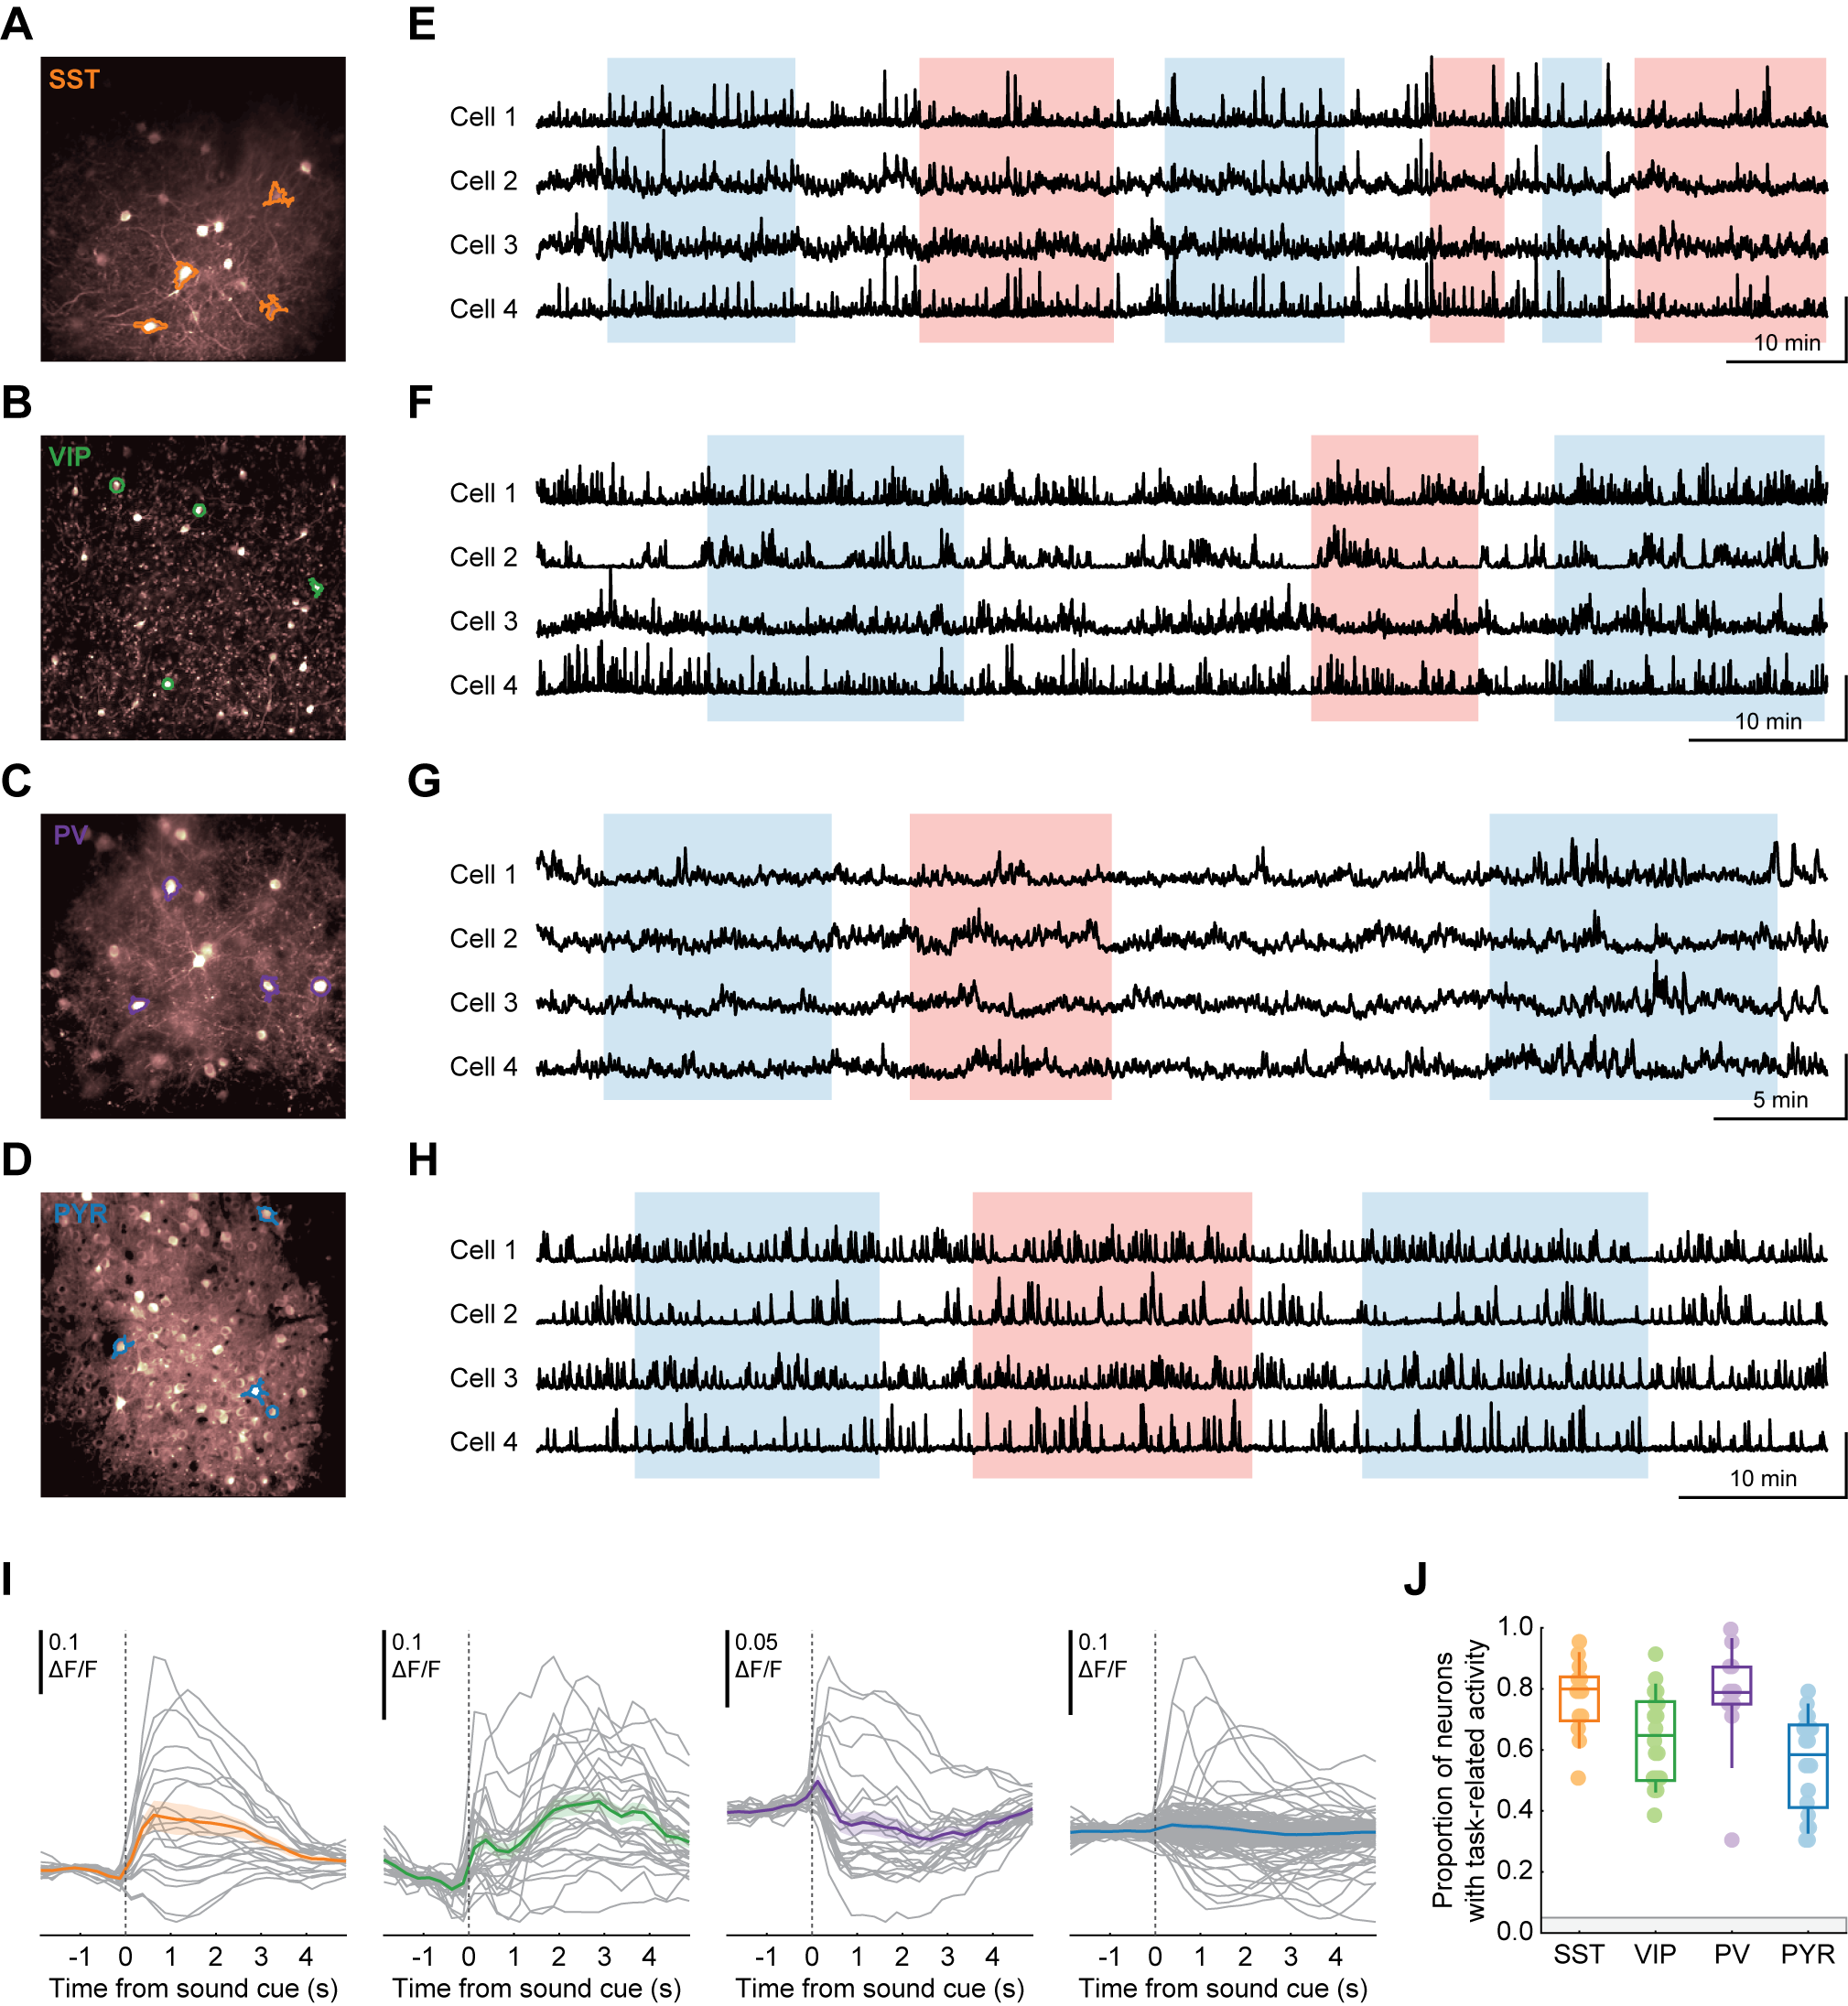
\includegraphics[width=\textwidth]{Figures/Chapter4/Fig4} 
\end{center}

\caption[Task-related neural activity in SST, VIP, PV, and PYR neurons]
{Task-related neural activity in SST, VIP, PV, and PYR neurons. (A--D) Mean projections from example fields-of-view showing SST, VIP, PV, and PYR neurons, respectively. (E--H) Example $\frac{\Delta F}{F}$ traces from the sessions in A--D. Red and blue background shading correspond to the action-left and action-right rule, respectively. White background indicates periods governed by the sound rule. Vertical scale bar, 1 SD (I) Mean $\frac{\Delta F}{F}$ traces from the sessions shown in E--H, presented as a function of time relative to the sound cue. Grey lines represent the mean trace for each neuron across all completed trials, re-centered on the mean value obtained during the pre-cue period. The grand $\mathit{mean} \pm \mathit{SEM}$ across all cells is overlaid in color. (J) Proportion of task-modulated neurons within each cell type, across $N=$ 13, 19, 12, and 20 sessions from SST, VIP, PV, and PYR neurons, respectively.}

\label{fig:Fig4}
\end{figure}